Getwork is a RPC method used by miners for retrieving block headers to find a solution for, or sending valid proofs of work; it was designed and introduced by the user called m0mchil in 2010.\cite{m0mchilbitcoingetwork}
Getwork was implemented in Bitcoin Core on 23rd November 2010: it's possible to read the official announcement regarding the Bitcoin Core update by Satoshi on BitcoinTalk Forum. \cite{bitcointalkGetwork}

\begin{figure}[h!]
    \centering
    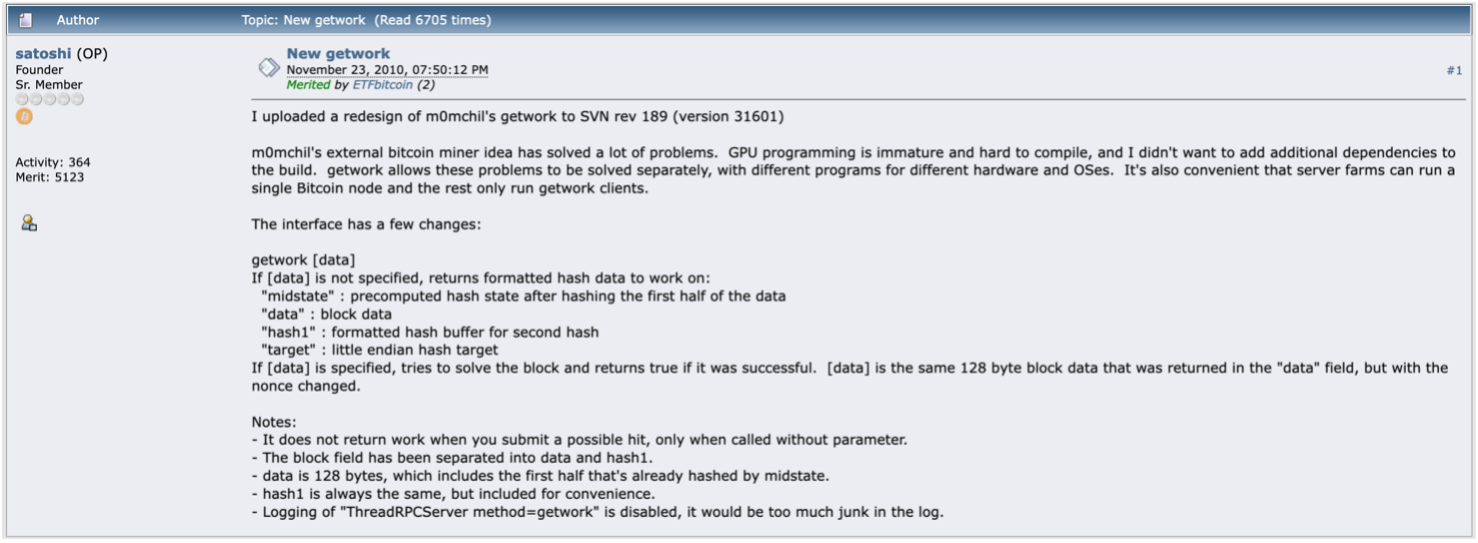
\includegraphics[width=15cm]{Figures/getwork/getwork1.png}
    \caption{Satoshi \textit{getwork} update announcement, Bitcoin Talk Forum}
    \label{fig:getwork1}
\end{figure}

\noindent The idea behind the getwork method was born by m0mchil's project called POCLbm (PyOpenCL bitcoin miner), the first open-source GPU miner software ever developed. \cite{m0mchilpoclbm}\\\\
Before entering the details of the getwork method, a reminder of the block header structure is needed, as represented in Figure \ref{fig:getwork2}.  

\begin{figure}[h!]
    \centering
    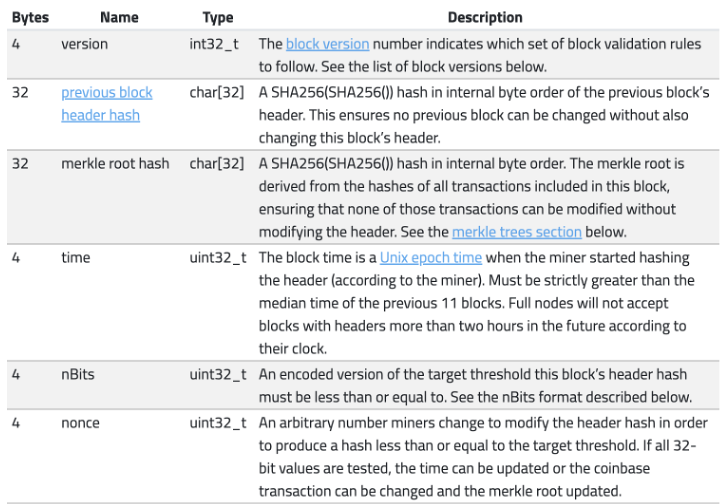
\includegraphics[width=15cm]{Figures/getwork/getwork2.png}
    \caption{Bitcoin block header fields, \textit{from \cite{bitcoinblockheader}}}
    \label{fig:getwork2}
\end{figure}

\noindent \textbf{NOTE:} Data present in the block header are all represented in little-endian order, except for the hashes (Hash of previous block's header and Merkle root) which are in internal-byte order (the original order of the SHA256 output, which can be considered little-endian as well).\\

\begin{figure}[h!]
    \centering
    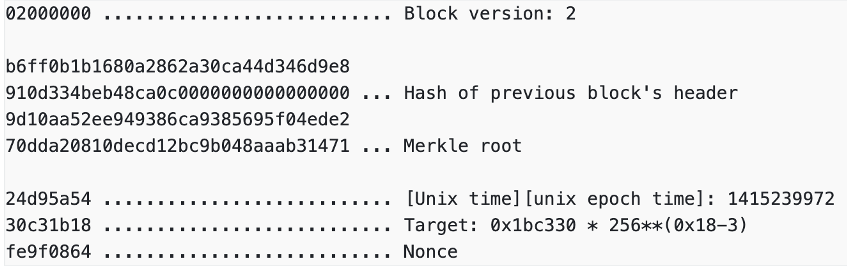
\includegraphics[width=15cm]{Figures/getwork/getwork3.png}
    \caption{Example Bitcoin block header, in hexadecimal format}
    \label{fig:getwork3}
\end{figure}

\noindent Considering the example in Figure \ref{fig:getwork3}, hash of previous block's header is represented in its internal byte order, but if you want to look for the corresponding block using a blockchain explorer, you must transform it to the RPC Byte Order (big-endian), obtaining this: \textbf{00000000000000000cca48eb4b330d91e8d946d344ca\\302a86a280161b0bffb6}.
The block corresponding to this hash is the one at height 328733. \cite{block328733} \begin{comment}, it can be deeply analyzed at \href{https://mempool.space/block/00000000000000000cca48eb4b330d91e8d946d344ca302a86a280161b0bffb6?showDetails=true#details}{https://mempool.space/block/00000000000000\\000cca48eb4b330d91e8d946d344ca302a
86a280161b0bffb6?showDetails=true\#de\\tails}.\end{comment}

\noindent For any further clarifications, on the BTC Information website can be found a complete documentation about the differences between internal-byte order and RPC Byte Order. \cite{btcinformationByteOrder} 